\chapter{Architecture}

Now that we understand the background and use case of Pepr3D, we can propose a software architecture for the project.
In this chapter, we show an overview of the whole architecture.
Further details are then available in next chapters.

\section{Overview}

\begin{figure}[b]
	\centering
	\centerline{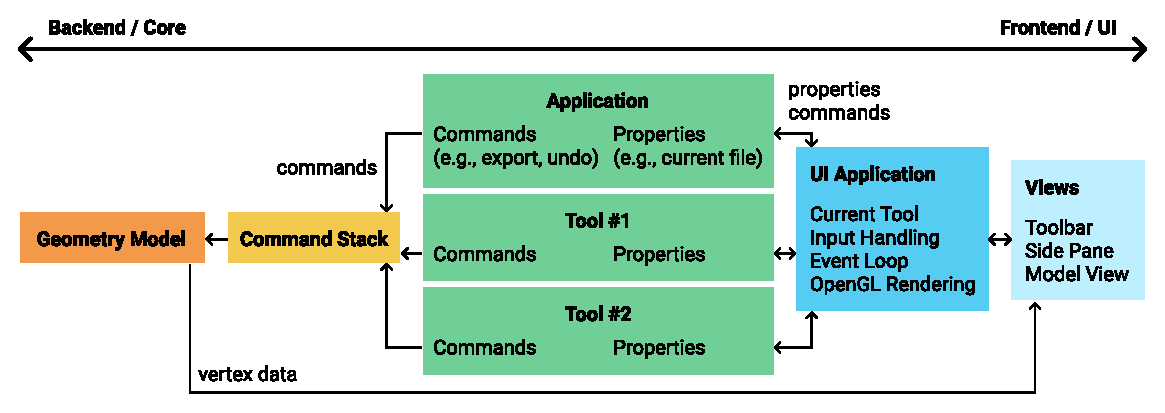
\includegraphics[scale=0.9]{images/architecture.eps}}
	\caption{An overview of the Pepr3D architecture.}
	\label{fig:architecture}
\end{figure}

A good software architecture should be easy to maintain and refactor, it should be possible to replace parts of it with new ones.
It should be as simple as possible, resistant to bugs and errors, and programs built with such architecture should run reasonably fast without any major bottlenecks.

This can be achieved with \emph{modularity}, i.e., separating a project into multiple parts that are as independent as possible.
It is important to define data flows and dependencies between the modules.
Keeping the data flows and dependencies as simple as possible makes it easy to replace modules in case it is necessary, e.g., when a certain library is not developed anymore or new technology is created.

\medskip

In our case, we tried to come up with a modular and simple architecture.
As Pepr3D is a 3D editor, it consists of both a complex \emph{backend} with geometry manipulation, and a complex \emph{frontend} for displaying and editing this geometry by a user.
We propose an architecture consisting of several parts ranging from backend to frontend. Details are in Figure~\ref{fig:architecture} and in the next section.

\section{Modules}

For the Pepr3D architecture, we propose the following modules:
%
\begin{itemize}
\item We need a module responsible for the geometry of the edited 3D object, including importing, exporting, and editing the object.
      \textbf{Geometry model} is a data structure describing everything Pepr3D needs to know about the 3D model.
      A 3D view is also rendered based on this structure.
\item Then we need a module allowing \emph{undo} and \emph{redo} functionality.
      In editors, this is mostly done using a \emph{command pattern}, in our case encapsulated in the \textbf{command stack} module.
      This module receives commands and changes the geometry model accordingly.
\item The commands are created and sent either directly from the \textbf{application} module or from \textbf{tools}.
      Application is responsible for generic commands such as loading and saving files, importing and exporting, or invoking undo and redo.
      Tools are responsible for their corresponding actions such as changing a color of a triangle or running a segmentation.
      Both application and tools also have \emph{properties}, e.g., a brush size of a brush tool.
\item The application and tools are managed by a \textbf{UI application} module which is a bridge between what the user sees and what the application does.
      It manages a window, handles events such as user input, processes asynchronous events in the event loop, manages an OpenGL context, etc.
\item Finally, \textbf{views} are responsible for actually displaying information on user's screen.
      They describe a toolbar, side pane, and a 3D model view.
      They correspond to buttons, text inputs, icons, numerical sliders, etc.
      The user interacts with Pepr3D through the views.
\end{itemize}

\section{Data flow}

In software such as editors, when we interact with the application, data first flow from frontend to backend (1.), and then from backend to frontend again (2.).

\paragraph{1. Front to back}

In our case, when a user uses a certain tool, e.g., a brush, and paints on the 3D model, this painting gets first registered in a \textbf{view}.
An asynchronous event is created through the \textbf{UI application} and a corresponding command is invoked from a current \textbf{tool} according to its properties.
The command is processed through the \textbf{command stack} to allow us to undo it in the future.
The command then modifies the \textbf{geometry model} accordingly.

\paragraph{2. Back to front}

After changing the \textbf{geometry model}, the command gets resolved and the \textbf{command stack} saves it to its history.
If no other commands are required by the \textbf{tool}, it notifies the \textbf{UI application} that the asynchronous event has finished.
The new geometry data are then immediately visible in the \textbf{view}, which renders the new geometry model.

\section{Choosing a language}

When selecting a programming language for a certain project, there are basically two important things to consider.
First, do we already have experience with the language or at least with a similar one?
Second, does this language provide all features necessary for the project?
Are there libraries available to help us building the software?
Is it not too complicated for the use case?

The first question is important because building a big project with a brand new language is very difficult.
It is too easy to start with a project and halfway through find out that one has been using the language concepts wrong the whole time.
We should have at least one person with some experience before starting.

The second part is important as some languages might be better for certain use cases.
For example, it would not make much sense making a web application in C++ instead of JavaScript, and vice-versa for complex geometry applications.

\medskip

In our case, we had quite a lot of experience with C++, C\#, JavaScript, and Python.
We want Pepr3D to be cross-platform and do heavy manipulations with 3D geometry as fast as possible.
We prefer compiled languages with optimized compilers, complex debuggers, profilers, and fast 3D libraries.

Other 3D editors are mostly developed with C++ and most suitable libraries (see section \ref{libs}) also primarily target C++.
It is also a language with cross-platform heavily optimized compilers.
Hence, we decided to choose \textbf{C++} as a primary language for Pepr3D.

\section{Dependencies}

In software development, it is a good idea \emph{not} to reinvent the wheel.
It means that if there is a library available for a certain task that we would like to do, it makes sense to consider using such library.

\subsection{Why yes, why not}

Libraries are useful for solving complex error-prone tasks that might be too difficult to implement ourselves.
As libraries typically have other users, there is a chance they have already spotted important bugs and reported them.
Hence there is a high chance they have already been fixed, which is not the case when we decide to develop our brand new custom solution.
Also, when a library is actively developed, it can keep improving and we do not even need to touch it.

Obviously, for certain tasks, a library might not exist, it might be too old and not maintained anymore, or it might not be in a good condition in general.
Using third party libraries makes maintenance of the project more difficult.
We need to keep checking if our dependencies are up to date, if there are known bugs or security issues in them.
Also in case we need to modify the library, we need to keep our custom fork of it and keep merging latest changes.
Different libraries also tend to use their own classes and structures for the same thing, which makes the source codes more difficult to understand.

\subsection{Libraries used by Pepr3D modules} \label{libs}

We have made a list of libraries that we would like to use to implement Pepr3D.
Details about why we have decided to use exactly \emph{these} libraries are available in specific chapters related to the modules.
This is just a brief overview:
%
\begin{itemize}
\item \textbf{Assimp}\footnote{http://www.assimp.org/} library should be used for importing and exporting 3D models for the \emph{Geometry Model} module.
\item \textbf{Cereal}\footnote{https://uscilab.github.io/cereal/} library should be used for (de)serialization of \emph{Geometry Model} and \emph{Application} data.
\item \textbf{CGAL}\footnote{https://www.cgal.org/} library is considered for complex 3D geometry and topology calculations in the \emph{Tools} commands affecting the \emph{Geometry Model}.
\item \textbf{Cinder}\footnote{https://libcinder.org/} library will be used in the \emph{UI Application} for managing cross-platform windows, input handling, asynchronous event loop, \textbf{OpenGL} context handling, and other related tasks.
\item \textbf{Dear ImGui}\footnote{https://github.com/ocornut/imgui} library will be used in \emph{Views} as a UI widgets library for managing buttons, text inputs, checkboxes, and other UI widgets.
\item This list of dependencies may not be final.
      Other libraries are also considered, such as \textbf{spirit-po}\footnote{https://github.com/cbeck88/spirit-po} for translating UI into different languages.
\end{itemize}
